\documentclass[10pt,aspectratio=169]{beamer}
\usepackage{metrobridge}

\usepackage{chronology}
\usepackage{subcaption}

\usepackage{appendixnumberbeamer}
\usepackage{minted}
\setminted{escapeinside=||,linenos,breaklines,autogobble}

\usepackage[backend=biber, citestyle=authortitle, maxbibnames=99]{biblatex}
\renewcommand{\cite}{\footcite}
\renewcommand{\footnotesize}{\fontsize{6pt}{6pt}\selectfont}
\addbibresource{references.bib}

\title{Performance and Dynamism in User-extensible Compiler Infrastructures}
\date{June 19th 2025}
\author{Edmund Goodman, co-supervised by Sasha Lopoukhine and Dr Tobias Grosser}

\begin{document}

\maketitle

\begin{frame}{The modern compiler designer's challenge}
    \begin{figure}[H]
        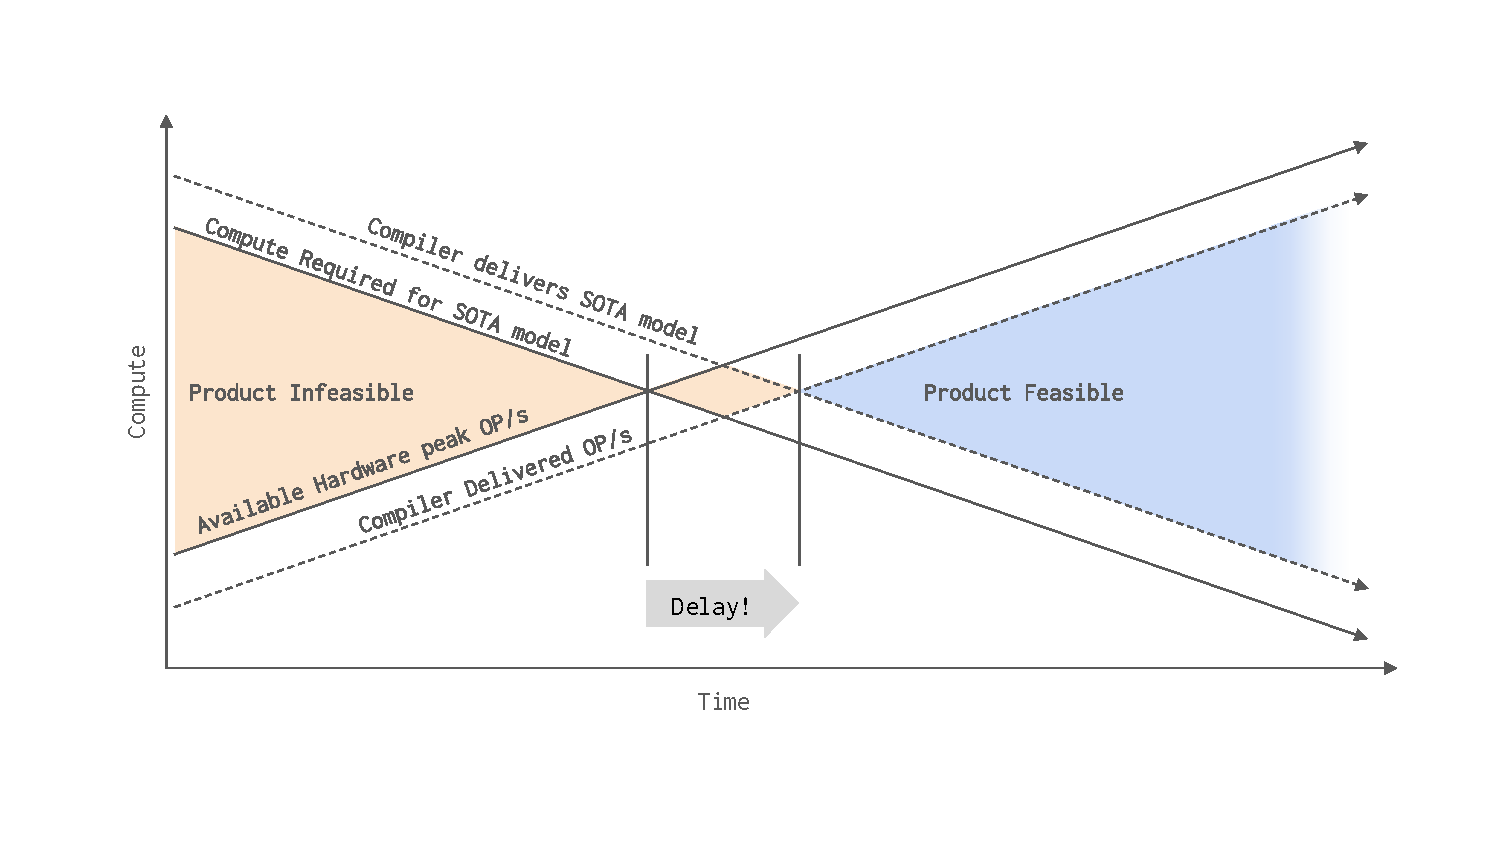
\includegraphics[width=0.8\textwidth]{images/compilers_lagging.pdf}
        \caption{Compilers are lagging behind the development of both machine
learning hardware and workloads. Figure created by Anton Lydike based on
a slide from a talk by Sean Silva’s talk\cite{seansilvaHighVelocityArchitectureMLIR2025}.}
        \label{fig:compilers_lagging}
    \end{figure}
\end{frame}

\begin{frame}[fragile]{An abridged history of compilers}
    \vspace{3em}
    \begin{chronology}*[5]{1950}{2025}{\textwidth}
        \event{1952}{A-0 System \cite{knuthEarlyDevelopmentProgramming1980}}%
        \event{1987}{GCC \cite{stallmanUsingGnuCompiler2009}}%
        \event{2002}{LLVM \cite{lattnerLLVMCompilationFramework2004}}%
        \event{2020}{MLIR \cite{lattnerMLIRScalingCompiler2021a}}%
        \event{2023}{xDSL \cite{fehrXDSLSidekickCompilation2025}}%
    \end{chronology}
    \vspace{1em}
\end{frame}

\begin{frame}[fragile]{MLIR \cite{lattnerMLIRScalingCompiler2021a}}
    \begin{columns}[T,onlytextwidth]
        \column{0.5\textwidth}
            {\large \vspace{0.5em} \textbf{``A compiler infrastructure\\ for the 
            end of Moore's law''} \vspace{0.5em}}
            \vspace{1.25em}
            \begin{itemize}
                \itemindent=-13pt
                \item User-defined dialects
                \item Common shared infrastructure
                \item Highly optimised C++
                \begin{itemize}
                    \itemindent=-13pt
                    \item[$\Rightarrow$] Slow to build, but fast to run
                \end{itemize}
            \end{itemize}
        \column{0.5\textwidth}
            \begin{listing}[H]
                \centering
                \begin{minted}[fontsize=\scriptsize,xleftmargin=3em]{text}
                    builtin.module {
                      %0 = arith.constant 865 : i32
                      %1 = arith.constant 395 : i32
                      %2 = arith.addi %1, %0 : i32
                      %3 = arith.constant 777 : i32
                      %4 = arith.addi %3, %2 : i32
                      "test.op"(%4) : (i32) -> ()
                    }
                \end{minted}
                \caption{A program amenable to constant folding, expressed in MLIR's textual IR.}
                \label{listing:mlir-ir}
            \end{listing}
    \end{columns}
\end{frame}

\begin{frame}{xDSL \cite{fehrXDSLSidekickCompilation2025}}
    \begin{columns}[T,onlytextwidth]
        \column{0.5\textwidth}
            \vspace{2em}
            {\large \textbf{A Python-native compiler framework, re-implementing MLIR’s data structures and logic}}
            \vspace{1.5em}
            \begin{itemize}
                \itemindent=-13pt
                \item Side-kick compiler for MLIR
                \item Runtime-extensible
                \item Readable Python
                \begin{itemize}
                    \itemindent=-13pt
                    \item[$\Rightarrow$] Fast to build and write, but slow to run?
                \end{itemize}
            \end{itemize}
        \column{0.5\textwidth}
            \begin{figure}[H]
                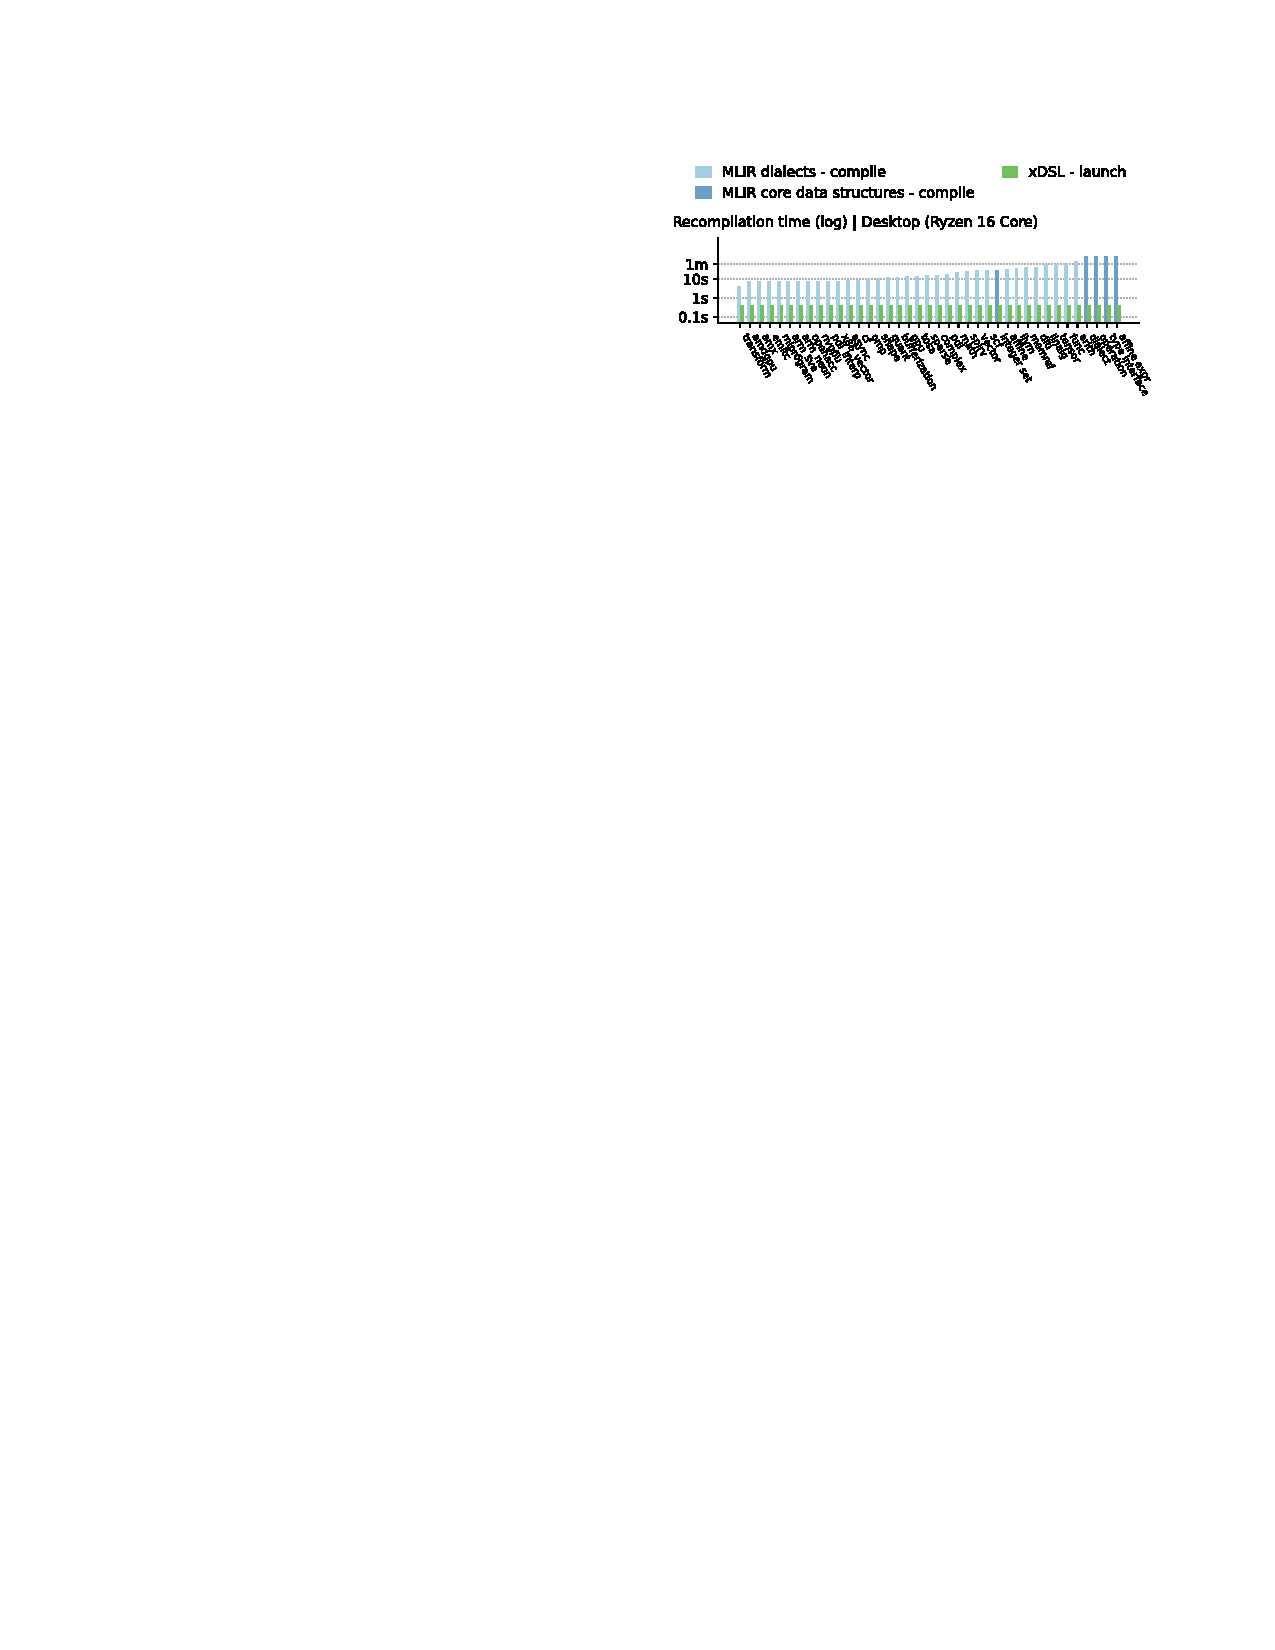
\includegraphics[width=\textwidth]{images/compile_times.pdf}
                \caption{``Recompiling MLIR after a single change is up
to two orders of magnitude slower than launching xDSL,
impacting prototyping and development efficiency'', Figure from xDSL paper \textsuperscript{8}.}
                \label{fig:compile_times}
            \end{figure}
    \end{columns}
\end{frame}

\begin{frame}{Key idea}
    \begin{center}
        \huge Pointer-chasing, unstructured workloads are hard to optimise ahead-of-time
    \end{center}
    \vspace{1em}
    \begin{itemize}
        \item Pointer-chasing workloads are bottlenecked by memory accesses\cite{wangEvaluatingSynchronizationOverhead2025}
        \item Runtime control flow incurs overhead and precludes optimisations \cite{driesenDirectCostVirtual1996}  \cite{emerybergerPythonPerformanceMatters2022}
        \item \textit{MLIR and xDSL are both examples of this workload type}
    \end{itemize}
\end{frame}

\begin{frame}{Research question}
    \begin{center}
        \huge How much does writing your compiler in a dynamic language actually slow it down? \\
    \end{center}
    \vspace{1.5em}
    \begin{itemize}
        \item Let's measure this, using MLIR and xDSL as proxies for static and dynamic languages
        \item Is this slow-down matched by other benefits of dynamic languages?
    \end{itemize}
\end{frame}

\begin{frame}{Contributions}
    \Large
    \begin{enumerate}
        \item Comparison of MLIR and xDSL performance
        \vspace{0.5em}
        \item Tool to examine Python at the bytecode level
        \vspace{0.5em}
        \item Impact of dynamic optimisations on xDSL
        \vspace{0.5em}
        \item Cost of dynamism for compiler frameworks
    \end{enumerate}
\end{frame}

\begin{frame}{Performance of MLIR and xDSL}
    \begin{columns}[T,onlytextwidth]
        \column{0.5\textwidth}
            \begin{itemize}
                \vspace{2em}
                \itemindent=-13pt
                \item Measure with micro-benchmarks \cite{aminiHowSlowMLIR2024}, and end-to-end optimisation workloads
                \vspace{1.5em}
                \item Current xDSL $100\times$ slower than MLIR
                \begin{itemize}
                    \itemindent=-13pt
                    \item Also measures implementation details
                \end{itemize}
                \item Specialised xDSL $14\times$ slower than MLIR
                \begin{itemize}
                    \itemindent=-13pt
                    \item Proxy for static and dynamic languages
                \end{itemize}
                \item Contrast $60,000\times$ slower for GEMM \cite{emerybergerPythonPerformanceMatters2022}
            \end{itemize}
            \vspace{1em}
        \column{0.5\textwidth}
            \vspace{1em}
            \begin{figure}[H]
                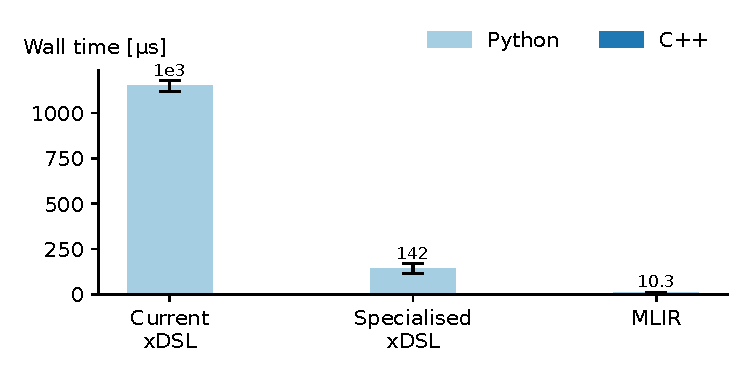
\includegraphics[width=\textwidth]{images/constant_performance.pdf}
                \caption{Performance of constant folding over twenty integer additions.}
                \label{fig:constant_performance}
            \end{figure}
    \end{columns}
\end{frame}

\begin{frame}[fragile]{Examining Python bytecode}
    \begin{figure}[H]
        \centering
        \begin{subfigure}[b]{0.275\textwidth}
           \centering
            \begin{minted}[fontsize=\scriptsize]{python}
    import bytesight
    
    def inner_function(x):
        assert x
    
    def example_function():
        inner_function(1)
    
    bytesight.profile_bytecode(
        example_function
    )
            \end{minted}
            \footnotesize\vspace{2em}
            \caption{Python program.}
            \label{listing:profiler-example-python}
        \end{subfigure}
        \hfill
        \begin{subfigure}[b]{0.7\textwidth}
            \centering
            \begin{minted}[fontsize=\scriptsize,linenos=false]{text}
    // ======= example:6 `example_function` ========
    // >>> inner_function(1)
    7           0   LOAD_GLOBAL          0   (inner_function) // 15 ns
                2   LOAD_CONST           1   (1)              // 15 ns
                4   CALL_FUNCTION        1   ()               // 31 ns
        // ======== example:3 `inner_function` =========
        // >>> assert x
        4           0   LOAD_FAST            0   (x)          // 13 ns
                    2   POP_JUMP_IF_TRUE     4   (to 8)       // 13 ns
                >>  8   LOAD_CONST           0   (None)       // 12 ns
                    10  RETURN_VALUE             ()           // 31 ns
        // =============================================
                6   POP_TOP                  ()               // 16 ns
                18  RETURN_VALUE             ()               // 28 ns
    // =============================================
            \end{minted}
            \caption{Profiler output.}
            \label{listing:profiler-example-bytecode}
        \end{subfigure}
        \vspace{-0.5em}
        \captionsetup{name=Listing}
        \caption{Our novel performance profiler, ByteSight, shows the sequence of dispatched bytecode and their individual execution times for Python programs.}
        \label{listing:profiler-example}
    \end{figure}
\end{frame}

\begin{frame}{Impact of dynamic optimisations on xDSL}
    \begin{columns}[T,onlytextwidth]
        \column{0.475\textwidth}
            \begin{itemize}
                \itemindent=-13pt
                \item Assess impact of CPython optimisations leveraging runtime information
                \item Use PyPerformance \cite{collinwinterPythonPyperformance2025} benchmarks as a baseline for average workloads
                \vspace{1em}
                \item xDSL yields $\sim5\%$ greater change than the average workload
                \item Specialised xDSL even more amenable to optimisation, up to $\sim11\%$ speedup
            \end{itemize}
        \column{0.025\textwidth}
        \column{0.5\textwidth}
            \begin{figure}[H]
                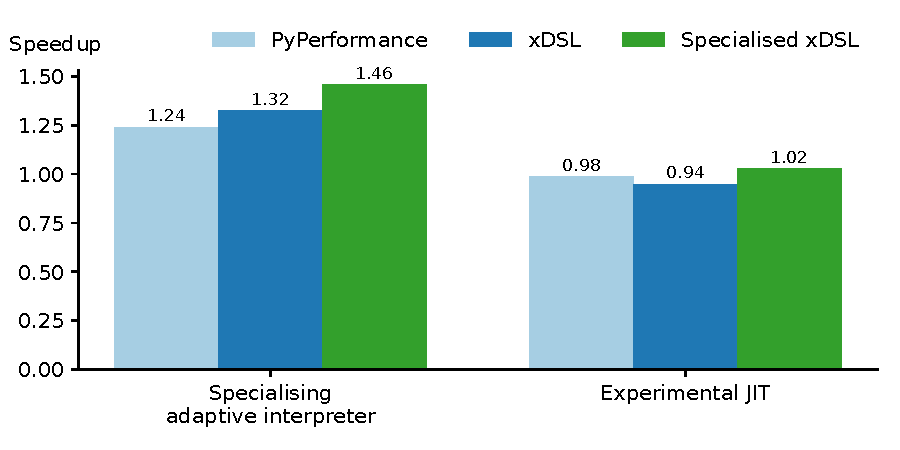
\includegraphics[width=\textwidth]{images/15_summary.pdf}
                \caption{Speed-up from optimisations across workloads.}
                \label{fig:15_summary}
            \end{figure}
    \end{columns}
\end{frame}

\begin{frame}{Cost of dynamism in compiler frameworks}
    \begin{columns}[T,onlytextwidth]
        \column{0.5\textwidth}
            \vspace{2em}
            \begin{figure}[H]
                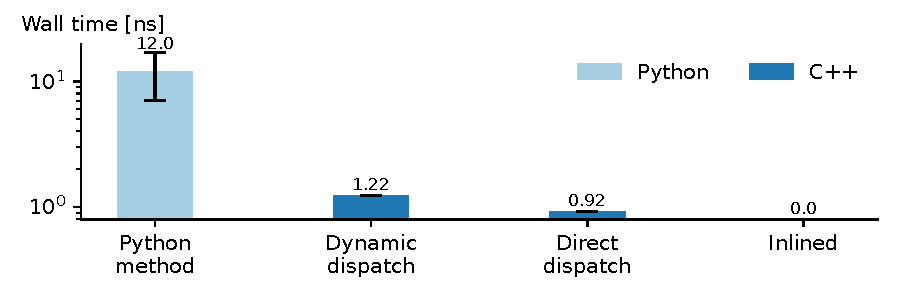
\includegraphics[width=\textwidth]{images/dispatch.pdf}
                \caption{Measuring dynamic function dispatch performance for Python 3.10 and \texttt{clang -O3}.}
                \label{fig:dispatch}
            \end{figure}
        \column{0.5\textwidth}
            \begin{itemize}
                \item Can quantify exact costs of specific dynamic components, for example
                \vspace{1em}
                \item C++ dynamic dispatch incurs overhead due to:
                \begin{enumerate}
                    \item Indirection through the vTable\cite{driesenDirectCostVirtual1996}
                    \item Precluding optimisations like function inlining
                \end{enumerate}
                \item Python dynamically dispatches all functions, incurring a high overhead
            \end{itemize}
    \end{columns}
\end{frame}

\begin{frame}{Conclusions}
    \begin{columns}[T,onlytextwidth]
        \column{0.5\textwidth}
            \vspace{3em}
            \begin{itemize}
                \itemindent=-13pt
                \item Compiler frameworks get less benefit out of ahead-of-time optimisations than more static workloads
                \item Dynamic languages provide other benefits, aiding development velocity
                \vspace{1.5em}
                \item \textit{Challenge the status quo of writing compiler frameworks in static languages}
            \end{itemize}
        \column{0.5\textwidth}
            \begin{figure}[H]
                \vspace{-1em}
                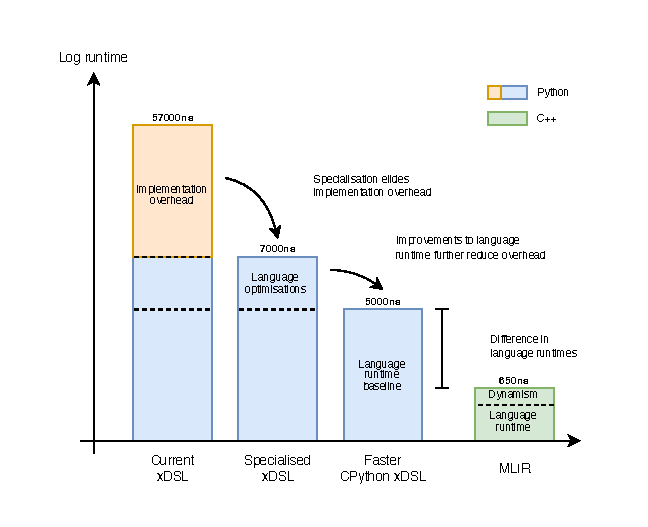
\includegraphics[width=\textwidth]{images/narrative.drawio.pdf}
                \vspace{-1.5em}
                \caption{Closing the gap between xDSL and MLIR pattern rewriting performance.}
                \label{fig:narrative}
            \end{figure}
    \end{columns}
\end{frame}

\begin{frame}{Impact and future work}
    \begin{figure}[H]
        \hspace*{-1cm}
        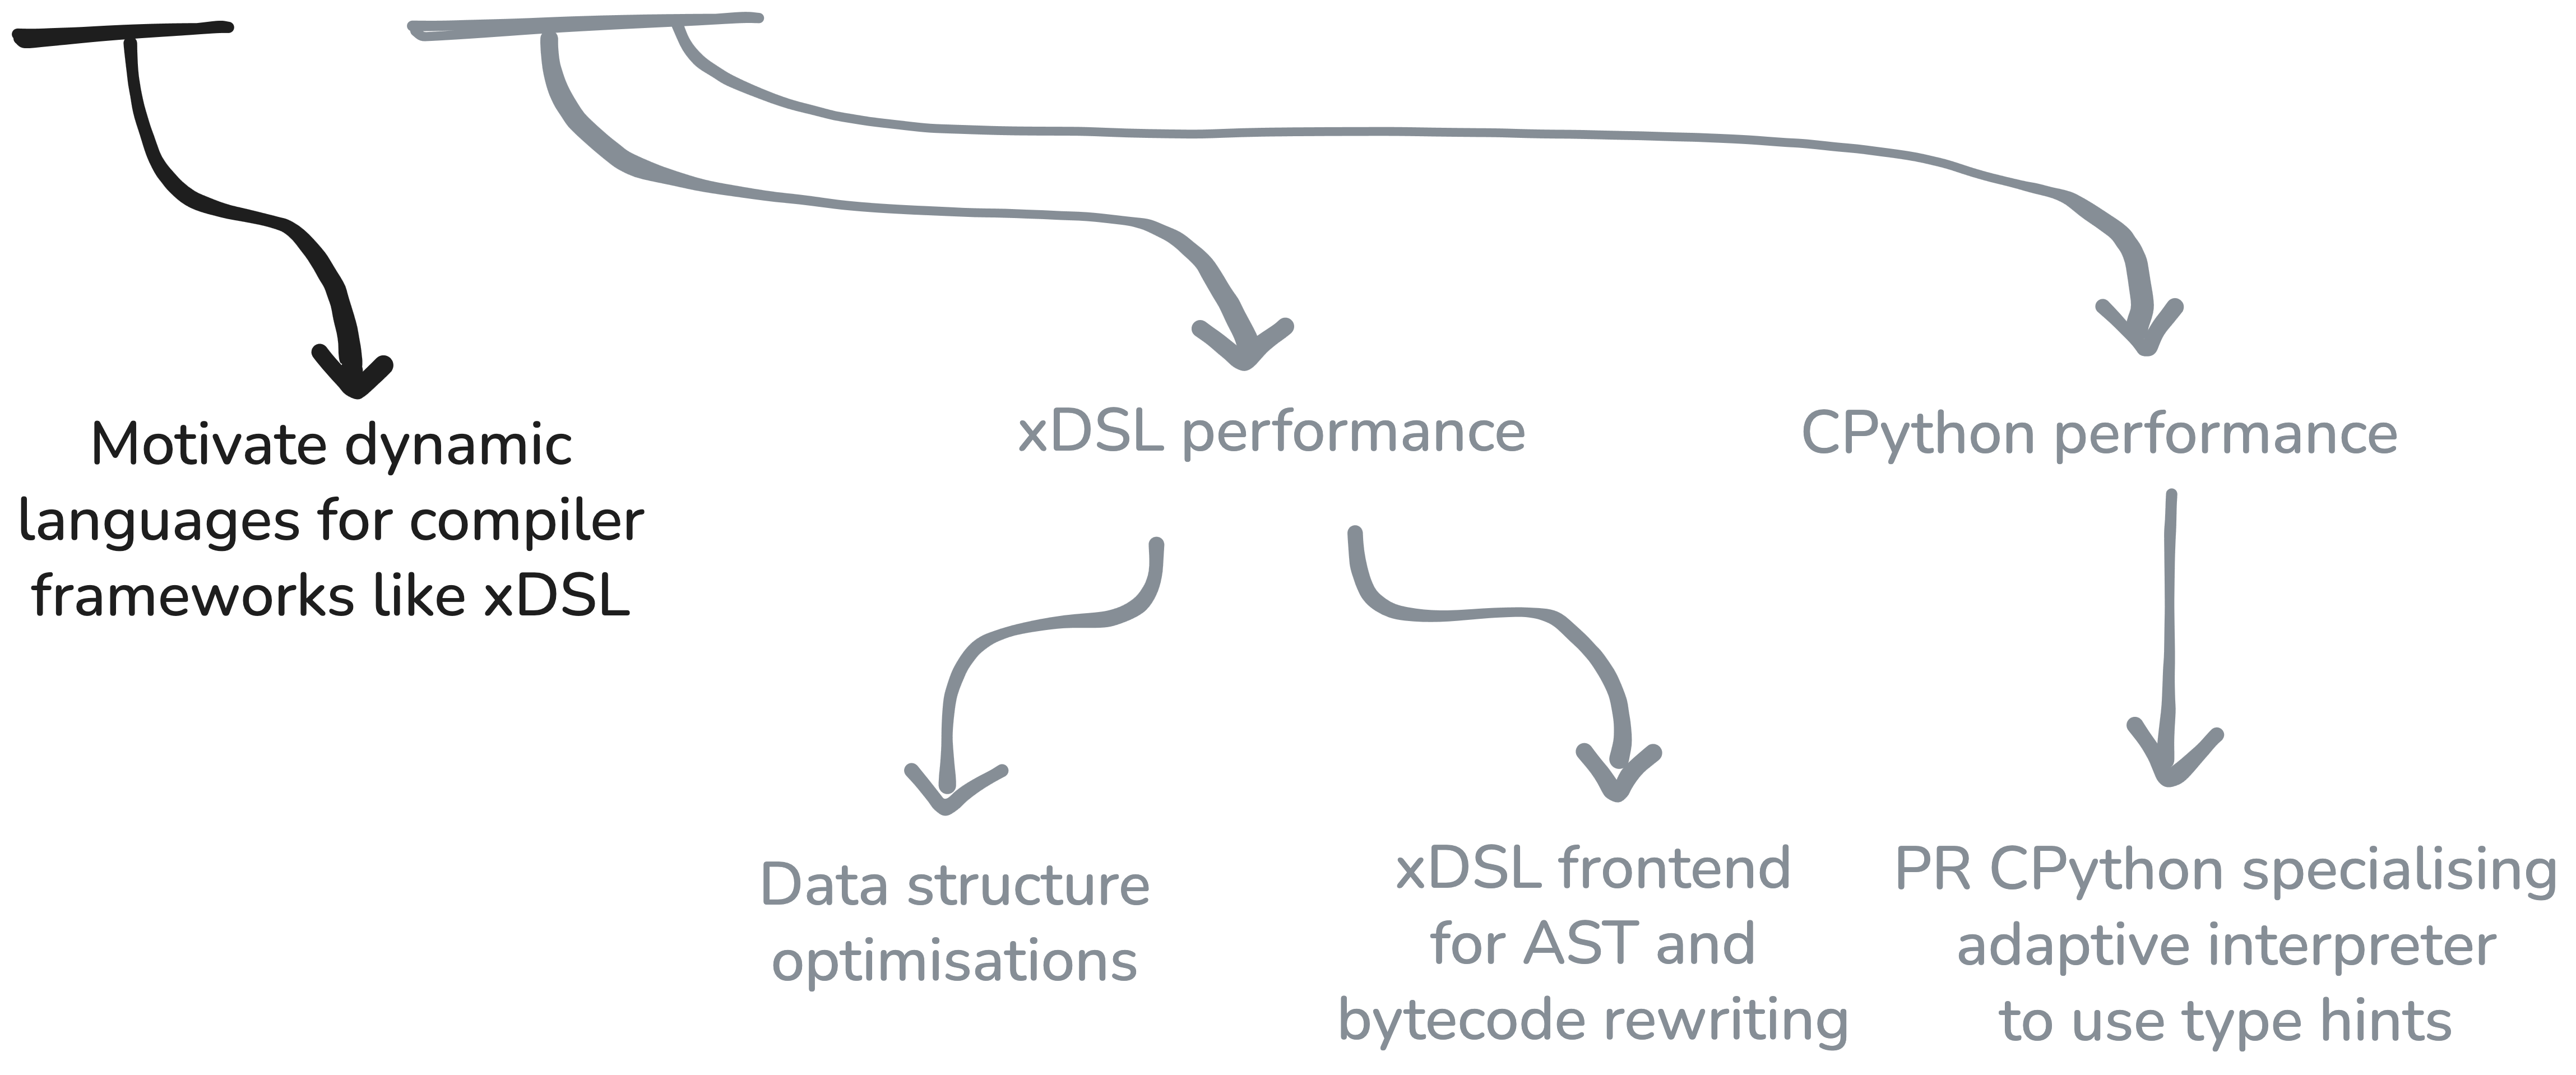
\includegraphics[width=\textwidth]{images/impact_future_work.png}
        \vspace{2cm}
    \end{figure}
\end{frame}

\appendix

\maketitle

\begin{frame}[allowframebreaks]{References}
    \printbibliography[heading=none]
\end{frame}

\end{document}